\documentclass{scrartcl}
\usepackage{etex}
\include{header/zusammenfassung}
\include{header/hyperref}
\include{header/listings}
\usepackage{tikz}
\usepackage{adjustbox}
\usetikzlibrary{arrows}
\usetikzlibrary{calc}
\usetikzlibrary{matrix}
\usetikzlibrary{intersections}

\newcommand\numberthis{\addtocounter{equation}{1}\tag{\theequation}}

\usepackage{circuitikz}
\usepackage{pgfplots}

\tikzstyle{3x3mask}=[
	matrix of nodes, 
	nodes={draw, minimum size=8mm, anchor=center},
	column sep=0mm
]


% Spaltenabstand bei ,ulticols
\setlength{\columnsep}{1.5em}

\title{DigPro2 Zusammenfassung}
\subtitle{Dozent: G.Schuster, Buch: Digital Image Processing, Rafael C. Gonzalez and Richard E.Woods}
\author{J. Rast, G. Köppel, R. Nestler, P. Riedel}

\begin{document}
\selectlanguage{english}

\lstset{language=Matlab}

\maketitle
\newpage

\tableofcontents
\newpage

\setcounter{section}{8}
\section{Morphological Image Processing\buch{Ch. 9}}

\subsection{Set Theory}
\begin{multicols}{2}
\subsubsection{Reflection}
\[
	\hat{B} = \{w | w = -b,\quad \text{for} \quad b \in B \}
\]


\subsubsection{Translation}
\[
	(B)_z = \{ c | c = b + z,\quad \text{for} \quad b \in B\}
\]


\subsubsection{Erosion}
With A and B as sets in $Z^2$, the erosion of A by B is defined as
\[
	A \ominus B = \{z|(B)_z \subseteq A  \}
\]

This is the set of all translations by z such that the set B is still a subset of A.

Equivalently, if B must be contained in A, it is not allowed to intersect with the background:
\[
	A \ominus B = \{z|(B)_z \cap A^c = \varnothing  \}
\]


\subsubsection{Dilation}
With A and B as sets in $Z^2$, the dilation of A by B is defined as
\[
	A \oplus B = \{z |(\hat{B})_z \cap A \neq \varnothing \}
\]
This is the set of all translations by z such that the set B reflected about its origin has at leas one overlap with the set A.

Equivalently, since the intersection is not allowed to be empty and all elements in it must be from A:
\[
	A \oplus B = \{z | [(\hat{B})_z \cap A] \subseteq A \}
\]


\subsubsection{Duality erosion/dilation}
Erosion and dilation are dual:
\[
	(A  \ominus B)^c = A^c \oplus \hat{B}
\]
\[
	(A \oplus B)^c = A^c \ominus \hat{B}
\]

\end{multicols}

\subsubsection{Opening and closing}
The opening of A by B is defined: (first erosion then dilation)
\[
	A \circ B = (A \ominus B) \oplus B
\]

The closing of A by B is defined: (first dilation then erosion)
\[
	A  \bullet B = (A \oplus B) \ominus B
\]

Opening and closing are dual operations: 
\[
	(A  \bullet B)^c = (A^c \circ \hat{B})
\]
\[
	(A \circ B)^c = (A^c \bullet \hat{B})
\]

\begin{figure}[h!]
	\centering
	\begin{subfigure}[b]{0.45\textwidth}
		\centering
		\adjustbox{scale=0.5}{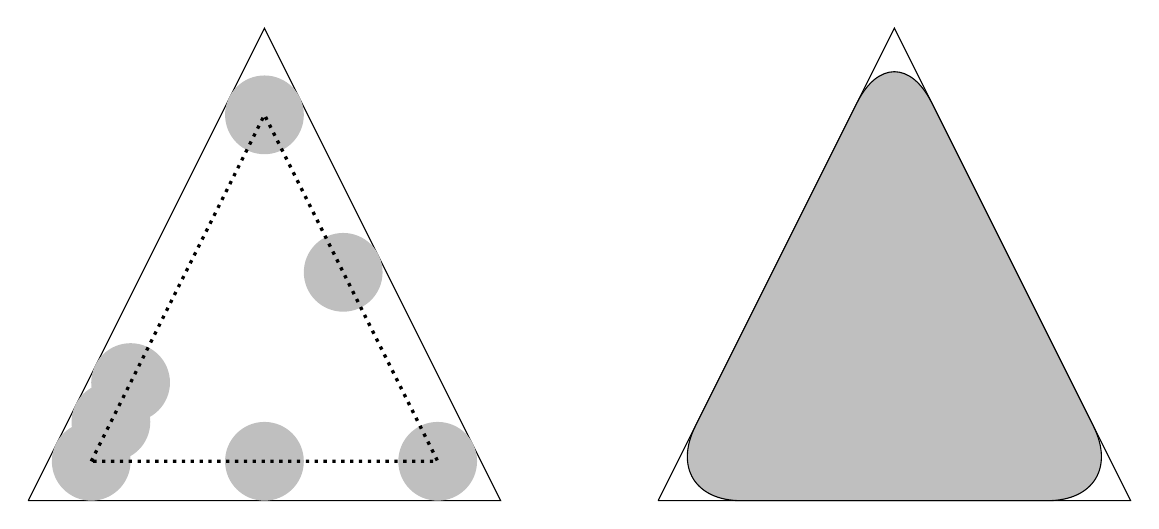
\begin{tikzpicture}
%linkes dreieck
\draw (0,0) -- (3,6) -- (6,0) -- (0,0);
\fill [lightgray] (0.8,0.5) circle (0.5);
\fill [lightgray] (1.05,1) circle (0.5);
\fill [lightgray] (1.3,1.5) circle (0.5);
\fill [lightgray] (3,4.9) circle (0.5);
\fill [lightgray] (4,2.9) circle (0.5);
\fill [lightgray] (5.2,0.5) circle (0.5);
\fill [lightgray] (3,0.5) circle (0.5);
\draw [dotted, very thick] (0.8,0.5) -- (3,4.9) -- (5.2,0.5) -- (0.8,0.5);

\draw (8,0) -- (11,6) -- (14,0) -- (8,0);
\draw [rounded corners=30pt, fill=lightgray] (9,2) -- (11,6) -- (14,0) -- (8,0) -- (9,2);

\end{tikzpicture}}
		\caption{Opening}
	\end{subfigure}
	\begin{subfigure}[b]{0.45\textwidth}
		\centering
		\adjustbox{scale=0.5}{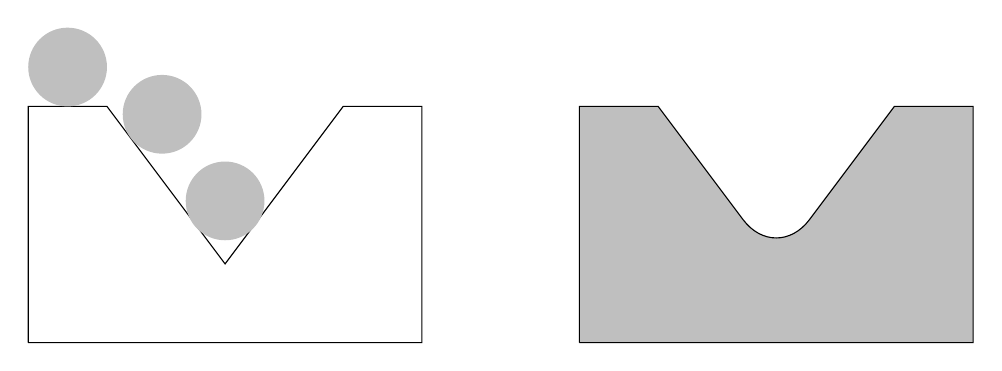
\begin{tikzpicture}

\draw (0,0) -- (0,3) -- (1,3) -- (2.5,1) -- (4,3) -- (5,3) -- (5,0) -- (0,0);
\fill [lightgray] (0.5,3.5) circle (0.5);
\fill [lightgray] (1.7,2.9) circle (0.5);
\fill [lightgray] (2.5,1.8) circle (0.5);

\draw [fill=lightgray] (7,0) -- (7,3) -- (8,3) [rounded corners=20pt] -- (9.5,1) [rounded corners=0] -- (11,3) -- (12,3) -- (12,0) -- (7,0);
\end{tikzpicture}}
		\caption{Closing}
	\end{subfigure}
	\caption{Geometrical interpretation of the opening and closing transformations}
\end{figure}


\subsubsection{The hit-or-miss transform}
The hit-or-miss transform is a basic tool for shape detection. Basic idea:
\begin{itemize}
	\item Through erosion of the image by the object, possible locations for the object in the image are left, since elements smaller than the objects disappear
	
	\item Through erosion of the background of the image with the local background of the object, possible locations for the object in the image are left
	
	\item The intersection of these possible locations result in a reliable  detection of the object location
	\[
		A \circledast B = (A \ominus D) \cap [ A^c \ominus (W-D)]
	\]
	
	\item In general, if B1 is the object and B2 is the corresponding background this can be written
	\[
		A \circledast B = (A \ominus B_1)\cap (A^c \ominus B_2)	
	\]	
\end{itemize}


\subsection{Some basic morphological algorithms}
\subsubsection{Convex hull}
\begin{itemize}
\item The convex hull H of a set S is the smalles convex set containing S.
\item H-S is called the convex deficiency of S
\end{itemize}
The convex hull is constructed with a convex hull with four structuring elements.
\begin{figure}[h]
	\centering
	\begin{subfigure}[b]{0.2\textwidth}
		\centering
		\adjustbox{scale=0.5}{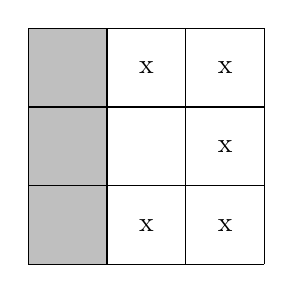
\begin{tikzpicture}
\draw [fill=lightgray] (0,0) rectangle  (1,3);
\foreach \x in {0,1,2,3} {
\draw (\x,0) -- (\x,3);
\draw (0,\x) -- (3,\x);}
\node at (1.5,0.5) {x};
\node at (2.5,0.5) {x};
\node at (2.5,1.5) {x};
\node at (2.5,2.5) {x};
\node at (1.5,2.5) {x};
\end{tikzpicture}}
		\caption{$B^1$}
	\end{subfigure}
	\begin{subfigure}[b]{0.2\textwidth}
		\centering
		\adjustbox{scale=0.5, angle=270}{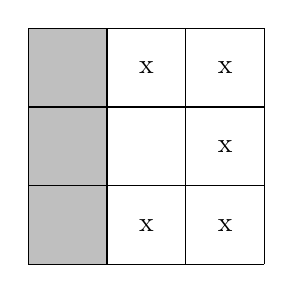
\begin{tikzpicture}
\draw [fill=lightgray] (0,0) rectangle  (1,3);
\foreach \x in {0,1,2,3} {
\draw (\x,0) -- (\x,3);
\draw (0,\x) -- (3,\x);}
\node at (1.5,0.5) {x};
\node at (2.5,0.5) {x};
\node at (2.5,1.5) {x};
\node at (2.5,2.5) {x};
\node at (1.5,2.5) {x};
\end{tikzpicture}}
		\caption{$B^2$}
	\end{subfigure}
	\begin{subfigure}[b]{0.2\textwidth}
		\centering
		\adjustbox{scale=0.5, angle=180}{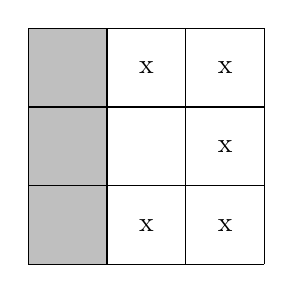
\begin{tikzpicture}
\draw [fill=lightgray] (0,0) rectangle  (1,3);
\foreach \x in {0,1,2,3} {
\draw (\x,0) -- (\x,3);
\draw (0,\x) -- (3,\x);}
\node at (1.5,0.5) {x};
\node at (2.5,0.5) {x};
\node at (2.5,1.5) {x};
\node at (2.5,2.5) {x};
\node at (1.5,2.5) {x};
\end{tikzpicture}}
		\caption{$B^3$}
	\end{subfigure}
	\begin{subfigure}[b]{0.2\textwidth}
		\centering
		\adjustbox{scale=0.5, angle=90}{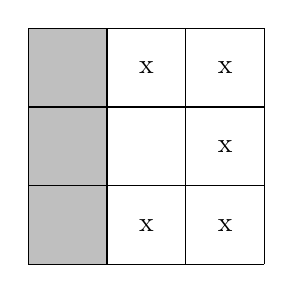
\begin{tikzpicture}
\draw [fill=lightgray] (0,0) rectangle  (1,3);
\foreach \x in {0,1,2,3} {
\draw (\x,0) -- (\x,3);
\draw (0,\x) -- (3,\x);}
\node at (1.5,0.5) {x};
\node at (2.5,0.5) {x};
\node at (2.5,1.5) {x};
\node at (2.5,2.5) {x};
\node at (1.5,2.5) {x};
\end{tikzpicture}}
		\caption{$B^4$}
	\end{subfigure}
	\caption{Structuring elements for convex hull}
\end{figure}

The resulting set is not the smallest convex set that contains A. The following additional constraints can be used:
\begin{itemize}
\item The convex hull is not allowed to grow beyond the original vertical and horizontal dimension
\item 
%TODO???
\end{itemize}

\subsubsection{Thinning}
Thinning is the operation of making the foreground thinner.
\begin{figure}[h]
	\centering
	\begin{subfigure}[b]{0.45\textwidth}
		\centering
		\adjustbox{scale=0.5}{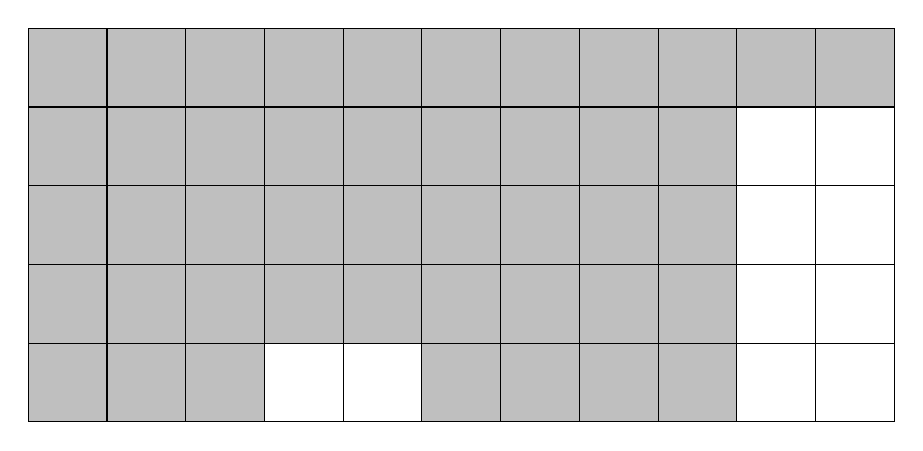
\begin{tikzpicture}
\draw[fill=lightgray] (0,5) rectangle (9,1);
\draw[fill=lightgray] (9,5) rectangle (11,4);
\draw[fill=lightgray] (5,1) rectangle (9,0);
\draw[fill=lightgray] (0,1) rectangle (3,0);
\foreach \x in {0,...,11} {
\draw (\x,0) -- (\x,5);}
\foreach \y in {0,...,5} {
\draw (0,\y) -- (11,\y);}
\end{tikzpicture}
}
		\caption{Original image}
	\end{subfigure}
	\begin{subfigure}[b]{0.45\textwidth}
		\centering
		\adjustbox{scale=0.5}{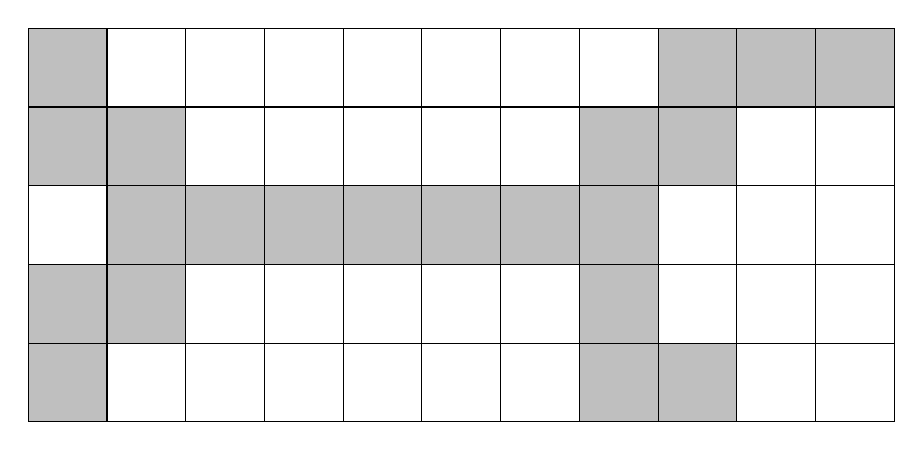
\begin{tikzpicture}
\draw[fill=lightgray] (1,3) rectangle (8,2);
\draw[fill=lightgray] (0,5) rectangle (1,4);
\draw[fill=lightgray] (0,4) rectangle (2,3);
\draw[fill=lightgray] (0,0) rectangle (1,1);
\draw[fill=lightgray] (0,1) rectangle (2,2);
\draw[fill=lightgray] (7,0) rectangle (9,1);
\draw[fill=lightgray] (7,1) rectangle (8,2);
\draw[fill=lightgray] (7,3) rectangle (9,4);
\draw[fill=lightgray] (8,4) rectangle (11,5);

\foreach \x in {0,...,11} {
\draw (\x,0) -- (\x,5);}
\foreach \y in {0,...,5} {
\draw (0,\y) -- (11,\y);}

\end{tikzpicture}}
		\caption{Thinned image}
	\end{subfigure}
	\caption{Thinning}
\end{figure}
	\[
		A \otimes  B = A - (A \circledast B)	
	\]	
Hit or miss transformation with rotating structuring elements.\\

\begin{figure}[h]
	\centering
	\begin{subfigure}[b]{0.1\textwidth}
		\centering
		\adjustbox{scale=0.5}{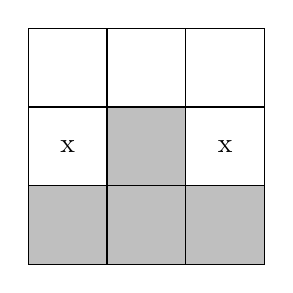
\begin{tikzpicture}
\draw [fill=lightgray] (0,0) rectangle  (3,1);
\draw [fill=lightgray] (1,1) rectangle  (2,2);
\foreach \x in {0,1,2,3} {
\draw (\x,0) -- (\x,3);
\draw (0,\x) -- (3,\x);}
\node at (0.5,1.5) {x};
\node at (2.5,1.5) {x};
\end{tikzpicture}}
		\caption{$B^1$}
	\end{subfigure}
	\begin{subfigure}[b]{0.1\textwidth}
		\centering
		\adjustbox{scale=0.5}{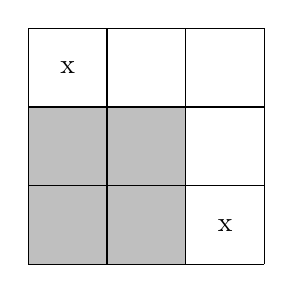
\begin{tikzpicture}
\draw [fill=lightgray] (0,0) rectangle  (2,2);
\foreach \x in {0,1,2,3} {
\draw (\x,0) -- (\x,3);
\draw (0,\x) -- (3,\x);}
\node at (0.5,2.5) {x};
\node at (2.5,0.5) {x};
\end{tikzpicture}}
		\caption{$B^2$}
	\end{subfigure}
	\begin{subfigure}[b]{0.1\textwidth}
		\centering
		\adjustbox{scale=0.5, angle=270}{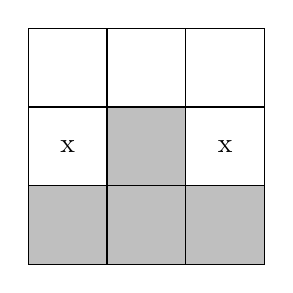
\begin{tikzpicture}
\draw [fill=lightgray] (0,0) rectangle  (3,1);
\draw [fill=lightgray] (1,1) rectangle  (2,2);
\foreach \x in {0,1,2,3} {
\draw (\x,0) -- (\x,3);
\draw (0,\x) -- (3,\x);}
\node at (0.5,1.5) {x};
\node at (2.5,1.5) {x};
\end{tikzpicture}}
		\caption{$B^3$}
	\end{subfigure}
	\begin{subfigure}[b]{0.1\textwidth}
		\centering
		\adjustbox{scale=0.5, angle=270}{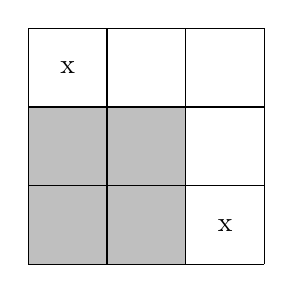
\begin{tikzpicture}
\draw [fill=lightgray] (0,0) rectangle  (2,2);
\foreach \x in {0,1,2,3} {
\draw (\x,0) -- (\x,3);
\draw (0,\x) -- (3,\x);}
\node at (0.5,2.5) {x};
\node at (2.5,0.5) {x};
\end{tikzpicture}}
		\caption{$B^4$}
	\end{subfigure}
	\begin{subfigure}[b]{0.1\textwidth}
		\centering
		\adjustbox{scale=0.5, angle=180}{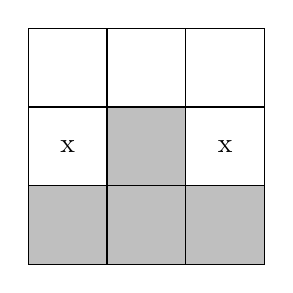
\begin{tikzpicture}
\draw [fill=lightgray] (0,0) rectangle  (3,1);
\draw [fill=lightgray] (1,1) rectangle  (2,2);
\foreach \x in {0,1,2,3} {
\draw (\x,0) -- (\x,3);
\draw (0,\x) -- (3,\x);}
\node at (0.5,1.5) {x};
\node at (2.5,1.5) {x};
\end{tikzpicture}}
		\caption{$B^5$}
	\end{subfigure}
	\begin{subfigure}[b]{0.1\textwidth}
		\centering
		\adjustbox{scale=0.5, angle=180}{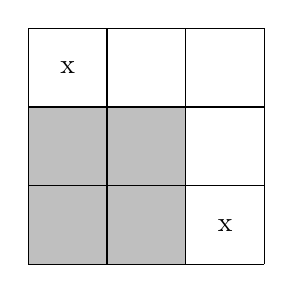
\begin{tikzpicture}
\draw [fill=lightgray] (0,0) rectangle  (2,2);
\foreach \x in {0,1,2,3} {
\draw (\x,0) -- (\x,3);
\draw (0,\x) -- (3,\x);}
\node at (0.5,2.5) {x};
\node at (2.5,0.5) {x};
\end{tikzpicture}}
		\caption{$B^6$}
	\end{subfigure}
	\begin{subfigure}[b]{0.1\textwidth}
		\centering
		\adjustbox{scale=0.5, angle=90}{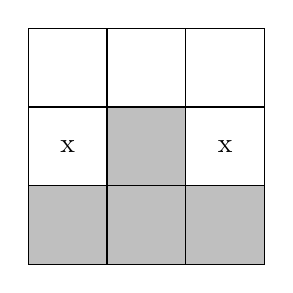
\begin{tikzpicture}
\draw [fill=lightgray] (0,0) rectangle  (3,1);
\draw [fill=lightgray] (1,1) rectangle  (2,2);
\foreach \x in {0,1,2,3} {
\draw (\x,0) -- (\x,3);
\draw (0,\x) -- (3,\x);}
\node at (0.5,1.5) {x};
\node at (2.5,1.5) {x};
\end{tikzpicture}}
		\caption{$B^7$}
	\end{subfigure}
	\begin{subfigure}[b]{0.1\textwidth}
		\centering
		\adjustbox{scale=0.5, angle=90}{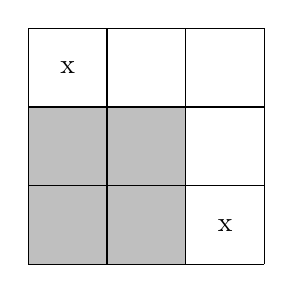
\begin{tikzpicture}
\draw [fill=lightgray] (0,0) rectangle  (2,2);
\foreach \x in {0,1,2,3} {
\draw (\x,0) -- (\x,3);
\draw (0,\x) -- (3,\x);}
\node at (0.5,2.5) {x};
\node at (2.5,0.5) {x};
\end{tikzpicture}}
		\caption{$B^8$}
	\end{subfigure}
	\caption{Thinning masks}
\end{figure}
	\[
		A \otimes  {B} = ((\ldots((A \otimes B^{1}) \otimes B^{2})\ldots) \otimes B^{n})	
	\]	

\subsubsection{Thickening}
This is the morphological dual of thinning. It is implemented as thinning the background and then taking the complement.

\subsubsection{Skeleton S(A)}
\begin{figure}[h!]
\centering
\begin{subfigure}[b]{0.45\textwidth}
\centering
\adjustbox{scale=0.5}{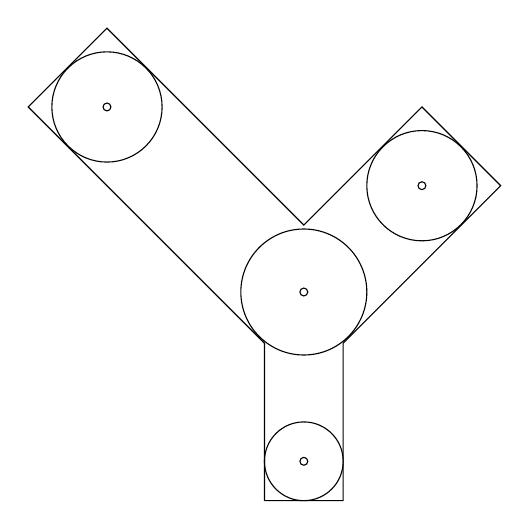
\begin{tikzpicture}
\draw (5,0) -- (6,0) -- (6,2) -- (8,4) -- (7,5) -- (5.5,3.5) -- (3,6) -- (2,5) -- (5,2) -- (5,0);
\draw (5.5,0.5) circle (0.5) circle (0.05);
\draw (3,5) circle (0.7) circle (0.05);
\draw (5.5,2.65) circle (0.8) circle (0.05);
\draw (7,4) circle (0.7) circle (0.05);
\end{tikzpicture}}
\caption{Positions of Maximum disks}
\end{subfigure}
\begin{subfigure}[b]{0.45\textwidth}
\centering
\adjustbox{scale=0.5}{\begin{tikzpicture}
\draw (5,0) -- (6,0) -- (6,2) -- (8,4) -- (7,5) -- (5.5,3.5) -- (3,6) -- (2,5) -- (5,2) -- (5,0);
\draw [dashed] (5,0) -- (5.5,0.5) -- (6,0);
\draw [dashed] (2,5) -- (3,5) -- (3,6);
\draw [dashed] (8,4) -- (7,4) -- (7,5);
\draw [dashed] (5.5,0.5) -- (5.5,2.65) -- (7,4);
\draw [dashed] (5.5,2.65) -- (3,5);
\end{tikzpicture}}
\caption{Complete Skeleton}
\end{subfigure}
\caption{Skeleton algorithm: basic idea}
\end{figure}
Finding a disk D that:
\begin{itemize}
\item centers at z
\item there is no larger disk containing D and included in A
\item touches the boundary of A at two or more places
\end{itemize}
	\[
		S(A) = \bigcup_{k=0}^{K} S_k(A)
	\]
with
	\[
		S_k(A) = (A \ominus kB) - (A \ominus kB) \circ B
	\]
	
\subsubsection{Pruning}
Pruning is a procedure that can remove parasitic components of a length below some threshold.\\
\begin{enumerate}
\item Find endpoints with a hit or miss transform with the following structuring elements. Remove the endpoints.
\begin{figure}[h!]
\centering
\begin{subfigure}[b]{0.45\textwidth}
\centering
\adjustbox{scale=0.5}{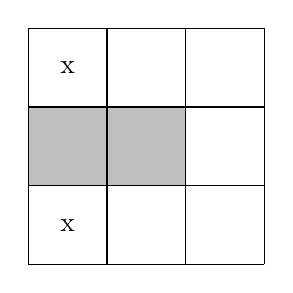
\begin{tikzpicture}
%\draw [fill=lightgray] (0,0) rectangle  (3,1);
\draw [fill=lightgray] (0,1) rectangle  (2,2);
\node at (0.5,0.5) {x};
\node at (0.5,2.5) {x};
\foreach \x in {0,1,2,3} {
\draw (\x,0) -- (\x,3);
\draw (0,\x) -- (3,\x);}
\end{tikzpicture}}
\caption{$B^1, B^2, B^3, B^4$ (rotated $90^\circ$)}
\end{subfigure}
\begin{subfigure}[b]{0.45\textwidth}
\centering
\adjustbox{scale=0.5}{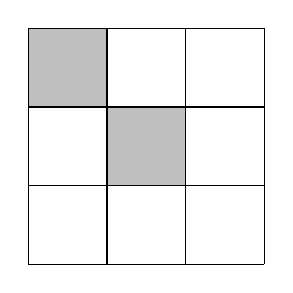
\begin{tikzpicture}
\draw [fill=lightgray] (0,3) rectangle  (1,2);
\draw [fill=lightgray] (1,1) rectangle  (2,2);
\foreach \x in {0,1,2,3} {
\draw (\x,0) -- (\x,3);
\draw (0,\x) -- (3,\x);}
\end{tikzpicture}}
\caption{$B^5, B^6, B^7, B^8$ (rotated $90^\circ$)}
\end{subfigure}
\caption{Pruning structuring elements}
\end{figure}
\item Repeat this. If you want to remove all spurs of length 3 or less, repeat for 3 times
\item Find the endpoints using the same structuring elements
\item Dilate the endpoints with a 3x3 structuring element and make a logical and with the original set
\end{enumerate}

\subsubsection{Geodesic dilation and erosion}
This is a transformation which uses two images and a structuring element
\begin{itemize}
\item F is the marker image
\item G is the mask image
\item Both are binary and F is a subset of G
\end{itemize}
\textbf{Geodesic dilation}
\[
	D_G^{(1)}(F) = (F\oplus B)\cup G
\]
Can be repeated:
\begin{align*}
	D_G^{(0)}(F) = F \\
	D_G^{(1)}(F) = (F\oplus B)\cup G\\
	D_G^{(n)}(F) = D_G^{(1)}[D_G^{(n-1)}(F)]
\end{align*}

\textbf{Geodesic erosion}
\[
	E_G^{(1)}(F) = (F\ominus B)\cap G
\]

\subsubsection{Morphological reconstruction}
This is geodesic dilation/erosion until nothing changes.

\subsubsection{Sample applications}
\textbf{Opening and closing by reconstruction}\\
Opening by reconstruction removes all small object, all others stay unchanged.
Closing by reconstruction closes gaps, the rest is unchanged. This is in contrast to morphological opening and closing, where the erosion removes the small objects and the dilation "sort of" reconstructs the other objects.\\

\textbf{Filling holes in a binary image I}\\
Without needing a seed!\\
\[
	H = [R_F^D(F)]^C
\]
\begin{figure}[h!]
\centering
\begin{subfigure}[b]{0.13\textwidth}
\centering
\adjustbox{scale=0.4}{\input{tikz/morphological/holefilling_I}}
\caption{$I$}
\end{subfigure}
\begin{subfigure}[b]{0.13\textwidth}
\centering
\adjustbox{scale=0.4}{\input{tikz/morphological/holefilling_Ic}}
\caption{$I^c$}
\end{subfigure}
\begin{subfigure}[b]{0.13\textwidth}
\centering
\adjustbox{scale=0.4}{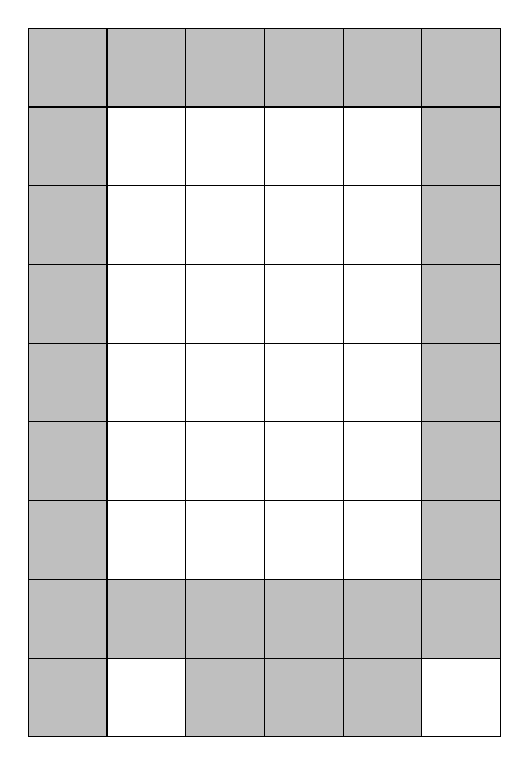
\begin{tikzpicture}
\draw [fill=lightgray] (0,0) rectangle (6,9);
\draw [fill=white] (1,2) rectangle  (5,8);
\draw [fill=white] (5,0) rectangle  (6,1);
\draw [fill=white] (1,0) rectangle  (2,1);

\foreach \x in {0,...,6} {
\draw (\x,0) -- (\x,9);}
\foreach \x in {0,...,9} {
\draw (0,\x) -- (6,\x);}
\end{tikzpicture}}
\caption{$F$}
\end{subfigure}
\begin{subfigure}[b]{0.13\textwidth}
\centering
\adjustbox{scale=0.4}{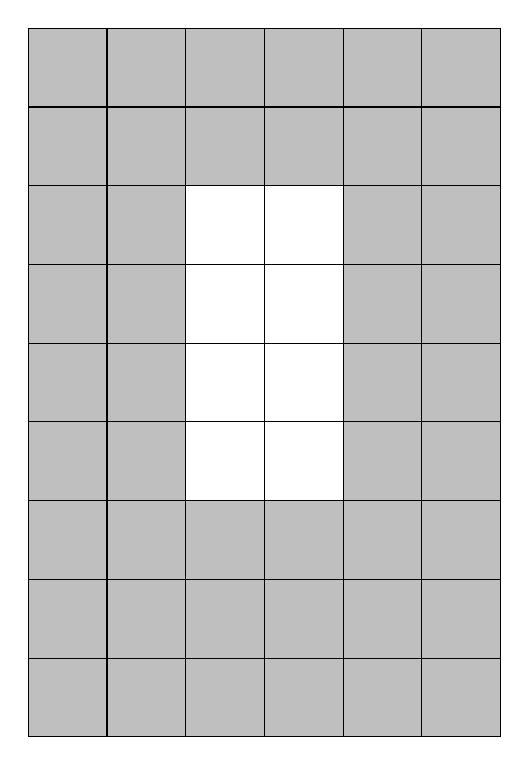
\begin{tikzpicture}
\draw [fill=lightgray] (0,0) rectangle (6,9);
\draw [fill=white] (2,3) rectangle  (4,7);

\foreach \x in {0,...,6} {
\draw (\x,0) -- (\x,9);}
\foreach \x in {0,...,9} {
\draw (0,\x) -- (6,\x);}
\end{tikzpicture}}
\caption{$C \oplus B$}
\end{subfigure}
\begin{subfigure}[b]{0.13\textwidth}
\centering
\adjustbox{scale=0.4}{\input{tikz/morphological/holefilling_FBIc}}
\caption{$C \oplus B \bigcap I^c$}
\end{subfigure}
\begin{subfigure}[b]{0.13\textwidth}
\centering
\adjustbox{scale=0.4}{\input{tikz/morphological/holefilling_H}}
\caption{$H$}
\end{subfigure}
\begin{subfigure}[b]{0.13\textwidth}
\centering
\adjustbox{scale=0.4}{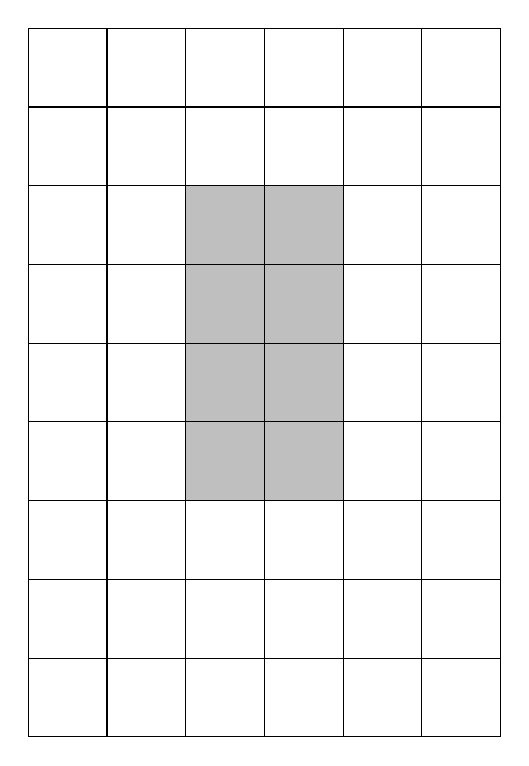
\begin{tikzpicture}
\draw [fill=lightgray] (2,3) rectangle  (4,7);

\foreach \x in {0,...,6} {
\draw (\x,0) -- (\x,9);}
\foreach \x in {0,...,9} {
\draw (0,\x) -- (6,\x);}
\end{tikzpicture}}
\caption{$H \bigcap I^c$}
\end{subfigure}
\caption{Hole Filling on a simple image}
\end{figure}

\textbf{Border clearing}\\
Remove object that touch the border.

\subsection{Gray-scale morphology}
The fundamental operations dilation, erosion, opening and closing can be extended to gray scale. Hence the more advanced operations which are based on the above operations can be extended too. The structuring elements are also gray-scale. In practice, flat structuring elements are preferred.

\begin{figure}[h!]
\centering
\begin{subfigure}[b]{0.45\textwidth}
\centering
\adjustbox{scale=0.5}{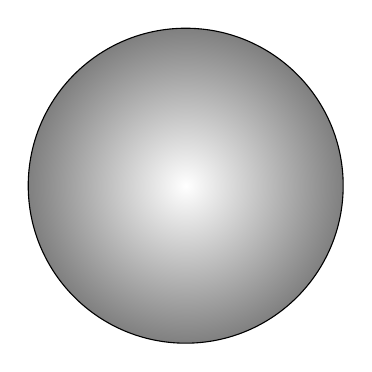
\begin{tikzpicture}
\draw [shading=radial, outer color=gray, inner color=white] (0,0) circle (2);\end{tikzpicture}}
\caption{Nonflat SE}
\end{subfigure}
\begin{subfigure}[b]{0.45\textwidth}
\centering
\adjustbox{scale=0.5}{\begin{tikzpicture}
\draw (0,0) circle (2);\end{tikzpicture}}
\caption{Flat SE}
\end{subfigure}\\
\begin{subfigure}[b]{0.45\textwidth}
\centering
\adjustbox{scale=0.5}{\begin{tikzpicture}
\draw (0,0) -- (0,2);
\draw (4,2) arc (0:180:2) ;
\draw (4,2) -- (4,0);
\end{tikzpicture}}
\caption{Intensity profile}
\end{subfigure}
\begin{subfigure}[b]{0.45\textwidth}
\centering
\adjustbox{scale=0.5}{\begin{tikzpicture}
\draw (0,0) -- (0,4) -- (4,4) -- (4,0);\end{tikzpicture}}
\caption{Intensity profile}
\end{subfigure}\\
\caption{Nonflat and flat structuring elements and corresponding horizontal intensity profiles through their center}
\end{figure}

Erosion
\[
	[f\ominus b](x,y) = \min_{(s,t)\epsilon b} \{f(x+s,y+t)\}
\]
Dilation
\[
	[f\oplus b](x,y) = \max_{(s,t)\epsilon b} \{f(x-s,y-t)\}
\]
Opening and closing are defined exactly the same as in the binary case.
\subsubsection{Morphological smoothing}
Opening suppresses bright details and closing suppresses dark details. They can be used in combination for image smoothing and/or noise suppression.
\subsubsection{Morphological gradient}
This operation resullts in an image where the edges are enhanced, not unlike a classical magnitude gradient image.
\[
	g=(f\oplus b)-(f\ominus b)
\]
\subsubsection{Top-hat transformation}
\[
	T_{hat}(f) = f -(f \circ b)
\]
The resulting image contains mostly bright details that are smaller than the structuring element.
\subsubsection{Bottom-hat transformation}
\[
	B_{hat}(f) = (f \circ b)-f
\]
The resulting image contains mostly dark details, that are smaller than the structuring element.
\subsubsection{Granulometry}
The goal of granulometry is to find the particle size distribution in an image. Opening with a structuring element similar in shape as the particles but the size scaled from small to large. The biggest effect in the resulting opened image is, when the size of the structuring element changes from just too small to just too large. This effect can be measured by summing up the entire opened image, the surface area. Jumps in the change of surface area show the dominant particle sizes.
\subsubsection{Textural segmentation}
Figure 9.43\\
The goal of textural segmentation is, to segment the image into two textural regions. The basic idea is to remove the small circles with a structuring element larger than the small circle but smaller than the large circle. With a following opening fills the white patches between the large elements.
\subsubsection{Gray-scale morphological reconstructions}
Follows the definition for binary images.\\
\textbf{Geodesic dilation of size 1}
\begin{align*}
	D_g^{(1)}(f) = (f\oplus b)\wedge g\\
	D_g^{(n)}(f) = D_g^{(1)}[D_g^{n-1}(f)] g
\end{align*}
$\wedge$ denotes the point-wise minimum operator\\
\textbf{Geodesic erosion of size 1}
\begin{align*}
	E_g^{(1)}(f) = (f\ominus b)\vee g\\
	E_g^{(n)}(f) = E_g^{(1)}[E_g^{(n-1)}(f)]
\end{align*}

\section{Image Segmentation}
\subsection{Preliminaries}
\begin{itemize}
\item Separate the image into different parts, ie. regions or objects
\item It is a difficult but important task
\item Often a scene can be designed that the segmentation task is simplified
\item Segmentation is based on some property of the scene
\begin{itemize}
\item Intensity discontinuity
\item Intensity similarity
\item More Complex properties:
\begin{itemize}
\item Motion
\item Texture
\item Shape
\item Color
\item etc.
\end{itemize}
\end{itemize}
\end{itemize}

\subsection{Fundamentals}
\begin{enumerate}
\item $\bigcup\limits_{i=1}^{n}R_i=R$
\item $R_i$ is a connected set, $i=1,2,...,n$
\item $R_i\bigcap R_j = $ for all $i$ and $j, i\neq j$
\item $Q(R_i)=$TRUE for $i=1,2,...n$
\item $Q(R_i\bigcup R_j)=$FALSE for any adjacent Regions $R_i$ and $R_j$
\end{enumerate}
Focus on the intenxity values
\begin{itemize}
\item there are discontinuities, then a new region starts.
\item If the intensity does not vary much, then this is one region.
\end{itemize}

\subsection{Point, line and edge detection}
When the intensity changes abruptly in a local neighborhood, this indicates an edge. It can be a simple point or a line.\\
Abrupt local changes can be detected using derivatives.\\
First order derivative
\[
	\frac{\partial f}{\partial x} = f'(x)=f(x+1)-f(x)
\]
The second order derivative
\[
	\frac{\partial^2f}{\partial x^2}=\frac{\partial f'(x)}{\partial x}=f''(x)=f(x+1)+f(x-1)-2f(x)
\]
This can be calculated using a spatial filter.
\[
	\begin{matrix}
	w_1, w_2, w_3\\
	w_4, w_5, w_6\\
	w_7, w_8, w_9
	\end{matrix}
\]
\begin{itemize}
\item First order in y direction $w_6=1, w_5=-1$
\item First order in x direction $w_8=1, w_5=-1$
\item Second order in y direction $w_6=1, w_4=1, w_5=-2$
\item Second order in x direction $w_8=1, w_2=1, w_5=-2$
\end{itemize}
\subsubsection{Detection of Isolated Points}
The Laplacian combines the second derivatives in both spatial directions. This results in
\[
	\nabla^2f(x,y)=f(x+1,y)+f(x-1,y)+f(x,y+1)+f(x,y-1)-4f(x,y)
\]
It can be extended to also include the diagonal terms wich results in the following mask
\[
	\begin{matrix}
	 1 & 1 & 1\\
	 1 & -8 & 1\\
	 1 & 1 & 1
	\end{matrix}
\]
The Laplacian is isotropic with respect to $0^\circ, 45^\circ, 90^\circ and 135^\circ$. 

\subsubsection{Line Detection}
Often, a line of a known direction should be detected. We use special masks for that particular direction
\begin{figure}[h]
	\centering
	\begin{subfigure}[b]{0.2\textwidth}
		\centering
		\[
		\begin{array}{|c|c|c|}
			\hline
			-1 & -1 & -1\\
			\hline
			2 & 2 & 2\\
			\hline
			-1 & -1 & -1\\
			\hline
		\end{array}
		\]
		\caption{Horizontal}
	\end{subfigure}
	\begin{subfigure}[b]{0.2\textwidth}
		\centering
		\[
		\begin{array}{|c|c|c|}
			\hline
			2 & -1 & -1\\
			\hline
			-1 & 2 & -1\\
			\hline
			-1 & -1 & 2\\
			\hline
		\end{array}
		\]
		\caption{$+45^\circ$}
	\end{subfigure}
	\begin{subfigure}[b]{0.2\textwidth}
		\centering
		\[
		\begin{array}{|c|c|c|}
			\hline
			-1 & 2 & -1\\
			\hline
			-1 & 2 & -1\\
			\hline
			-1 & 2 & -1\\
			\hline
		\end{array}
		\]
		\caption{Vertical}
	\end{subfigure}
	\begin{subfigure}[b]{0.2\textwidth}
		\centering
		\[
		\begin{array}{|c|c|c|}
			\hline
			-1 & -1 & 2\\
			\hline
			-1 & 2 & -1\\
			\hline
			2 & -1 & -1\\
			\hline
		\end{array}
		\]
		\caption{$+45^\circ$}
	\end{subfigure}
	\caption{Line detection masks}
\end{figure}
%TODO Seite 20 Figure 10.10

\subsubsection{Edge localization}
The previously shown method generates edge points. The goal is to keep the ones which truly belong to an edge.\\
Since first order derivatives are helpful, a nice way of combining the two partial derivatives into one value is the magnitude of the gradient
\begin{equation}
	\nabla f = grad(f) = \left[\begin{array}{c} g_x \\ g_y \end{array}\right] =  \left[\displaystyle{\begin{array}{c} \frac{\partial f}{\partial x} \vspace{0.2cm}  \\ \frac{\partial f}{\partial y} \end{array}}\right] \notag
\end{equation}

The gradient (which is a vector) points into the direction of the greatest rate of change of f at the location (x,y)\\
The magnitude of the gradient vector is the value of the rate of change in that direction\\
Gradient operators:\\
\begin{figure}[h]
	\centering
	\begin{subfigure}[b]{0.2\textwidth}
		\centering
		\[
		\begin{array}{|c|c|c|}
			\hline
			-1 & -1 & -1\\
			\hline
			0 & 0 & 0\\
			\hline
			1 & 1 & 1\\
			\hline
		\end{array}
		\]
		\caption{Prewitt}
	\end{subfigure}
	\begin{subfigure}[b]{0.2\textwidth}
		\centering
		\[
		\begin{array}{|c|c|c|}
			\hline
			-1 & 0 & 1\\
			\hline
			-1 & 0 & 1\\
			\hline
			-1 & 0 & 1\\
			\hline
		\end{array}
		\]
		\caption{Prewitt}
	\end{subfigure}
	\begin{subfigure}[b]{0.2\textwidth}
		\centering
		\[
		\begin{array}{|c|c|c|}
			\hline
			-1 & -2 & -1\\
			\hline
			0 & 0 & 0\\
			\hline
			1 & 2 & 1\\
			\hline
		\end{array}
		\]
		\caption{Sobel}
	\end{subfigure}
	\begin{subfigure}[b]{0.2\textwidth}
		\centering
		\[
		\begin{array}{|c|c|c|}
			\hline
			-1 & 0 & 1\\
			\hline
			-2 & 0 & 2\\
			\hline
			-1 & 0 & 1\\
			\hline
		\end{array}
		\]
		\caption{Sobel}
	\end{subfigure}
	\caption{Prewitt and Sobel masks}
\end{figure}\\
After the gradient images have been calculated, often the magnitude of the gradient is required.
\[
	M(x,y) \approx |g_x|+|g_y|
\]
If the goal is to find the dominant edges, then smoothing the image before calculating the magnitude gradient image works well. Alternatively, the magnitude gradient image can also be thresholded such that only values above this value are considered edges (set to one). Everything else is set to 0.

\subsubsection{Marr-Hildreth edge detector}
New Idea: Edges exist on different scales. The edge detector needs to be tuned to the scale of the desired edge. Use a Gaussian filter (with space constant $\sigma$) and then take the Laplacian. The Gaussian filter is a low pass, wich blurs the image for large $\sigma$. This results in a Laplacian of Gaussian (LoG) filter.
\begin{figure}[h]
	\centering
	\begin{subfigure}[b]{0.45\textwidth}
		\centering
		\adjustbox{scale=0.5}{\usetikzlibrary{arrows}
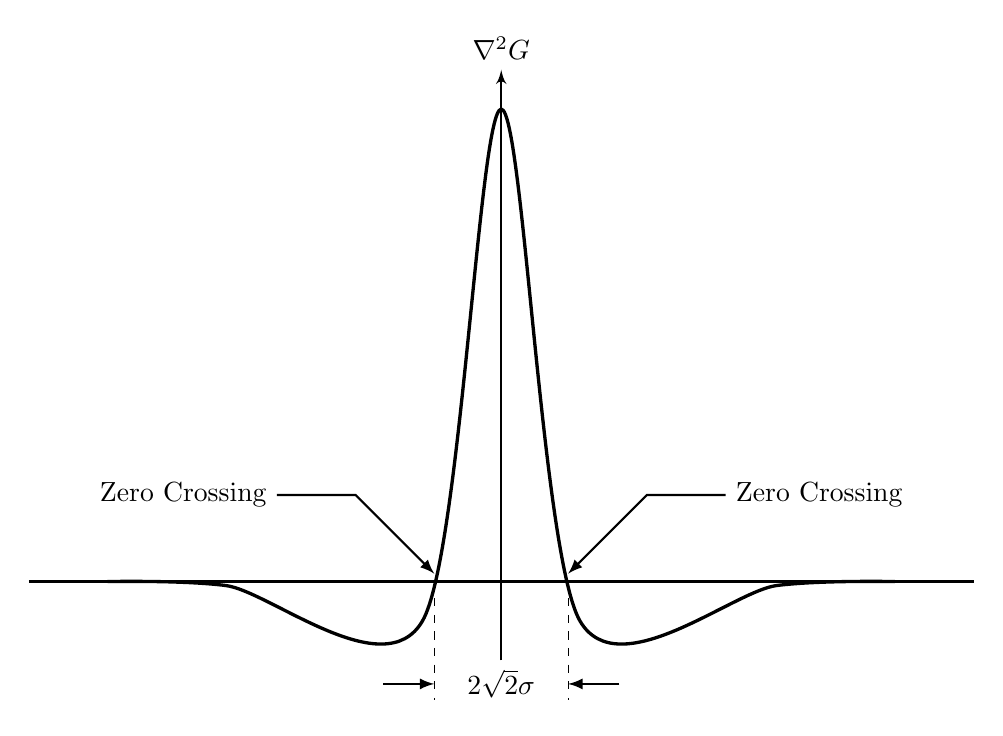
\begin{tikzpicture}
	\draw[thick] (-6,0) -- (6,0);
	\draw[thick, -latex'] (0,-1) -- (0, 6.5) node[above] {$\nabla^2G$};
	
	\draw[latex-, thick] (-.85,0.10) -- ++(-1,1) -- ++(-1,0) node[left] {Zero Crossing};
	\draw[latex-, thick] (.85,0.10) -- ++(1,1) -- ++(1,0) node[right] {Zero Crossing};
	
	\draw[dashed] (-.85, 0) -- (-.85, -1.5);
	\draw[dashed] (.85, 0) -- (.85, -1.5);
	\draw (0,-1.3) node {$2\sqrt{2}\sigma$};
	\draw[-latex, thick] (-1.5,-1.3) --(-.85 , -1.3);
	\draw[-latex, thick] (1.5,-1.3) --(.85 , -1.3);	

	\draw[very thick] plot [smooth] coordinates {(-5,0) (-3.5,-0.05) (-1,-0.5) (0,6) (1,-0.5) (3.5,-0.05) (5,0)};
\end{tikzpicture}}
		\caption{Cross Section of the negative of the LoG, showing zero crossings}
	\end{subfigure}
	\begin{subfigure}[b]{0.45\textwidth}
		\centering
		\adjustbox{scale=0.75}{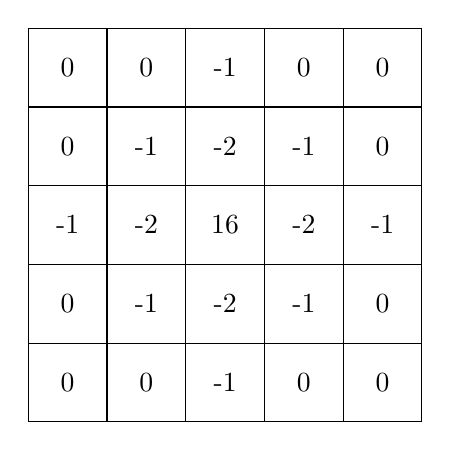
\begin{tikzpicture}

\foreach \x in {0,...,5} {
	\draw (\x,0) -- (\x,5);
	\draw (0,\x) -- (5,\x);
}

\foreach \x/\y in {0/0,1/0,0/1,3/0,4/0,4/1,0/3,0/4,1/4,3/4,4/4,4/3} {
	\node at  (\x+0.5,\y+0.5) {0};
}
\foreach \x/\y in {2/0,0/2,4/2,2/4,1/1,1/3,3/1,3/3} {
	\node at  (\x+0.5,\y+0.5) {-1};
}
\foreach \x/\y in {2/1,1/2,2/3,3/2} {
	\node at  (\x+0.5,\y+0.5) {-2};
}

\node at (2.5,2.5) {16};

\end{tikzpicture}}
		\caption{5x5 mask approximation. The negative of this mask would be used in practicej}
	\end{subfigure}
	\caption{Marr-Hildreth}
\end{figure}

\textbf{Summary of the Marr-Hildreth edge detection:}
\begin{enumerate}
\item Filter the input image with an $n x n$ Gaussian lowpass filter $G(x,y)=e^{-\frac{x^2+y^2}{2\sigma^2}}$
\item Compute the Laplacian of the image resulting from Step 1. $\nabla ^2[G(x,y) \star f(x,y)]$
\item Find the zero crossing of the image from Step 2.
\end{enumerate}
\textbf{Size of the discrete LoG filter}
Rule of thumb: nxn LoG filter should have the smallest odd integer n greater than or equal to $6\sigma$.\\
\textbf{How to find the zero crossings?}
A zero-crossing exists, if at least one opposing pixelpair has a sign difference.
%TODO Matrix edge detection
%*rx 
%o o
%xr*
%zwei paare davon müssen ein vorzeichen ändern

\subsubsection{Canny edge detector}
More complex, more powerful. The derivation is powerful, the implementation easy. Canny uses the gradient angle image and the linking of weak with strong edges.\\
Smooth the image and then find the gradient vector magnitude and direction:
\begin{align*}
G(x,y) = e^{-\frac{x^2+y^2}{2\sigma^2}}\\
f_s(x,y)=G(x,y)\star f(x,y)\\
M(x,y) = \sqrt{g_x^2+g_y^2}\\
\alpha(x,y) = tan^{-1}\left[\frac{g_y}{g_x}\right]\\
\end{align*}
The first new idea is, to thin the edges, using the gradient directional information. This is called nonmaxima suppression.\\
%TODO ?
We are looking for the maxima of the gradient magnitude along the gradient direction. $g_N(x,y)$ is the nonmaxima-suppressed image, the gradient magnitude image where the wide ridges have been thinned since the middle value is only kept when it is the maxima within a 3x3 neighborhood along the gradient direction.\\
This image is thresholded to find the significant edges and remove the noise.

\begin{itemize}
\item $T_H$ high threshold. The values above this are almost certainly true edges
\item $T_L$ low threshold. The values above this are likely to be edges. If they are 8-connected to a edge in $g_{NH}(x,y)$, they are also an edge.
\end{itemize}
%TODO Seite 50 summary canny

\subsubsection{Edge linking and boundary detection}
Three schemes to link edges:\\
\textbf{Local processing}\\
For every point at a location the gradient vector magnitude and angle are compared with the magnitude and angle of points in a neighborhood. If these are similar, they belong to the same boundary. This can be indicated by giving them the same color and/or gray value.\\
A much simpler scheme can be used if the linking follows certain directions and the maximum gap size is roughly known.\\
%TODO enumerate seite 55
\textbf{Regional processing}\\
If the location of a boundary is roughly known, it is possible to use the detected edge points as indicators for the suspected boundary.
\begin{enumerate}
\item Let P be a sequence of ordered, destinct, 1-valued points of a binary image. Specify two starting points, A and B. these are two starting vertices of the polygon.
\item Specify a threshold T, and two empty stacks, OPEN and CLOSED.
\item If the points in P correspond to a closed curve, put A into OPEN and put B into OPEN and CLOSED.
\item Compute the parameters of the line passing from the last vertex in CLOSED to the last vertex in OPEN.
\item Compute the distances from the line in Step 4 to all the points in P whose sequence places them between the vertices from Step 4. Select the point, $V_{max}$, with the maximum distance $D_{max}$ (ties are resolved arbitrarily)
\item If $D_{max}$, place $V_{max}$ at the end of the OPEN stack as a new vertex. Go to Step 4.
\item Else, remove the last vertex from Open and insert it as the last vertex of CLOSED.
\item If OPEN is not empty, go to Step 4.
\item Else, exit. The vertices in CLOSED are the vertices of the polygonal fit to the points in P.
\end{enumerate}
\begin{figure}[h]
	\centering
	\adjustbox{scale=0.5}{\usetikzlibrary{calc}
\begin{tikzpicture}[dot/.style={circle,inner sep=1pt, fill, name=#1}]

\begin{scope}[shift={(-5.5,1)}]
\node [dot=A] at (-2,-1.4) {};
\node [dot=B] at (-2.4,0.4) {};
\node [dot=C] at (1.2,-2.2) {};
\node [dot=D] at (2.2,-1.4) {};
\node [dot=E] at (2.6,-0.2) {};
\node [dot=F] at (2.4,0.8) {};
\node [dot=G] at (-1.6,1.8) {};
\node [dot=H] at (-2.2,1.2) {};
\node [dot=I] at (-2.4,-0.6) {};
\node [dot=J] at (2,1.6) {};
\node [dot=K] at (1.2,2) {};
\node [dot=L] at (0.4,2.4) {};
\node [dot=M] at (-0.8,2.2) {};
\draw[thick] (A) -- (C);
\draw[thick, dashed] ($(A)!(L)!(C)$) -- (L);
\end{scope}

\begin{scope}[shift={(0.9,1)}]
\node [dot=A] at (-2,-1.4) {};
\node [dot=B] at (-2.4,0.4) {};
\node [dot=C] at (1.2,-2.2) {};
\node [dot=D] at (2.2,-1.4) {};
\node [dot=E] at (2.6,-0.2) {};
\node [dot=F] at (2.4,0.8) {};
\node [dot=G] at (-1.6,1.8) {};
\node [dot=H] at (-2.2,1.2) {};
\node [dot=I] at (-2.4,-0.6) {};
\node [dot=J] at (2,1.6) {};
\node [dot=K] at (1.2,2) {};
\node [dot=L] at (0.4,2.4) {};
\node [dot=M] at (-0.8,2.2) {};
\draw[thick] (A) -- (L) -- (C);
\draw[thick, dashed] ($(A)!(H)!(L)$) -- (H);
\draw[thick, dashed] ($(L)!(F)!(C)$) -- (F);
\end{scope}

\begin{scope}[shift={(-5.5,-5)}]
\node [dot=A] at (-2,-1.4) {};
\node [dot=B] at (-2.4,0.4) {};
\node [dot=C] at (1.2,-2.2) {};
\node [dot=D] at (2.2,-1.4) {};
\node [dot=E] at (2.6,-0.2) {};
\node [dot=F] at (2.4,0.8) {};
\node [dot=G] at (-1.6,1.8) {};
\node [dot=H] at (-2.2,1.2) {};
\node [dot=I] at (-2.4,-0.6) {};
\node [dot=J] at (2,1.6) {};
\node [dot=K] at (1.2,2) {};
\node [dot=L] at (0.4,2.4) {};
\node [dot=M] at (-0.8,2.2) {};
\draw[thick] (A) -- (H) -- (L) -- (F) -- (C);
\draw[thick, dashed] ($(A)!(I)!(H)$) -- (I);
\draw[thick, dashed] ($(L)!(M)!(H)$) -- (M);
\draw[thick, dashed] ($(L)!(J)!(F)$) -- (J);
\draw[thick, dashed] ($(F)!(D)!(C)$) -- (D);
\end{scope}

\begin{scope}[shift={(0.9,-5)}]
\node [dot=A] at (-2,-1.4) {};
\node [dot=B] at (-2.4,0.4) {};
\node [dot=C] at (1.2,-2.2) {};
\node [dot=D] at (2.2,-1.4) {};
\node [dot=E] at (2.6,-0.2) {};
\node [dot=F] at (2.4,0.8) {};
\node [dot=G] at (-1.6,1.8) {};
\node [dot=H] at (-2.2,1.2) {};
\node [dot=I] at (-2.4,-0.6) {};
\node [dot=J] at (2,1.6) {};
\node [dot=K] at (1.2,2) {};
\node [dot=L] at (0.4,2.4) {};
\node [dot=M] at (-0.8,2.2) {};
\draw[thick] (A) -- (I) -- (H) -- (M) -- (L) -- (J) -- (F)-- (D) -- (C);
\end{scope}

\end{tikzpicture}}
	\caption{Regional Processing}
\end{figure}
\textbf{Global processing}\\
\subsubsection{Hough transform}
\begin{itemize}
%TODO Figure 10.31 Seite 63 und Bild Normale Seite 64
\item Each point in the xy plane belongs to infinetly many lines $y_i=ax_i+b$
\item If we interpret this line equation differently, then $b=-x_ia+y_i$ represent for each point in the xy plane a line in the ab plane
\item For each point in the xy plane, a line can be drawn in the ab plane and the principal lines in the xy plane can be found by the points with the most intersections in the ab plane
\item Vertical lines require an infinite a, this does not work. Use the line normal as representation. A point in the xy plane does not result in a simple straight line in the parameter space ($\theta\rho$). The curve $\rho = f(\theta)$ is now a sinusoidal
\item Practical scheme
\begin{itemize}
\item For every $\theta_q$ in the $\rho\theta$ plane
\item Calculate $\rho = f(\theta)$ and quantize it into $\rho_q$
\item Increase the cell in the $\rho\theta$ plane at location ($\rho_q, \theta_q$) by one
\item end
\end{itemize}
\end{itemize}

\subsection{Thresholding}
\subsubsection{Basic global thresholding}
\begin{equation}
g(x,y)=\begin{cases}1 \qquad \text{if } f(x,y) > T \\0 \qquad  \text{if } f(x,y) \leq T \end{cases} \label{thresholdingBasic}
\end{equation}

\begin{enumerate}
\item Select an initial estimate for the global threshold, T
\item Segment the image using T in Gleichung(\ref{thresholdingBasic}). This will produce two groups of pixels: $G_1$ consisting of all pixels with intensity values $> T$, and $G_2$ consisting of pixels with values $\leq T$
\item Compute the average (mean) intensity values $m_1$ and $m_2$ for the pixels in $G_1$ and $G_2$, repsectively
\item Compute a new threshold value: \begin{equation}
T=\frac{1}{2}(m_1+m_2)\notag
\end{equation} 
\item Repeat Steps 2 through 4 until the difference betwenn values of $T$ in successive iterations is smaller than a predefined paramter $\Delta T$
\end{enumerate}
\subsubsection{Optimum global thresholding using Otsu’s Method}

Two different variances are important
\begin{itemize}
\item Within-class variance
\item Between-class variance
\end{itemize}
\begin{eqnarray}
\sigma_W^2 = P_1\sigma_1^2+P_2\sigma_2^2 
& & \sigma_W \text{ Within-class variance} \notag \\
\sigma_B^2 = P_1(m_1-m_G)^2+P_2(m_2-m_G)^2
& & \sigma_B \text{ Between-class variance} \notag \\
\sum_{i=0}^{L-1} p_i = 1 
& & \notag \\
m_G=\sum_{i=0}^{L-1} i \ p_i 
& & m_G: \text{ global mean}  \notag \\
\sigma_G^2 = \sum_{i=0}^{L-1} (i-m_G)^2 p_i
& & \sigma_G \text{global variance} \notag \\
P_1(k) =\sum_{i=0}^{k} p_i
& &  P_1: \text{ probability of the background}   \notag \\
P_2(k)=\sum_{i=k+1}^{L-1}1-P_1(k)
& & P_2: \text{ probability of the object} \notag \\
m_1(k)=\frac{1}{P_1(k)}\sum_{i=0}^{k} i \ p_i
& &  m_1: \text{ mean intensity of the background}  \notag \\
m_2(k)=\frac{1}{P_2(k)}\sum_{i=k+1}^{L-1} i \ p_i 
& &  m_2: \text{ mean intensity of the object}  \notag \\
\sigma_B^2 = P_1(m_1-m_G)^2+P_2(m_2-m_G)^2 & &  \text{Using algebra to change the form} \notag \\
=P_1 P_2 (m_1-m_2)^2 = \frac{(m_G P_1 - m)^2}{P_1(1-P_1)} & & \notag \\
\sigma_B^2(K*)=\max\limits_{0\leq k \leq L-1} \sigma_B^2(K)
& & \text{Optimum of k for maximizing is } k* \notag \\
\eta(k)=\frac{\sigma_B^2(k)}{\Sigma_G^2}
& & 0 \leq  \eta(k*)\leq 1 \notag
\end{eqnarray}

\subsubsection{Variable Thresholding}
\textbf{Image Partitioning}\\
The simplest approach is to partition a given image into non overlapping regions and then use Otsu's method on smaller regions.\\
\textbf{Based on local image properties}\\
A threshold is computed for each point. The threshold depends on some property of a local neighborhood. Common properties are the mean and standard deviation for each pixel.
An even more powerful scheme can be built, if the 1 or 0 decision is based on some logical condition.\\

\subsection{Region based segmentation}
The goal is to segment the image into regions directly, not using abrupt changes or thresholding.
\subsubsection{Region growing}
\begin{enumerate}
\item Find all connected components in $S(x,y)$ and erode each connected component to one pixel; label all such pixels found as 1. All other pixels in S are labeled 0.
\item Form an image $f_Q$ such that, at a pair of coordinates...
%TODO Folie 104 Nr. 1 bis 4 schreiben
\end{enumerate}
\subsubsection{Region splitting and merging}
The image is subdivided initially into a set of arbitrary disjoint regions and then the regions are merge and or split in an attempt to improve the segmentation.\\
A common scheme to split images is a quadtree.\\
%TODO Seite 107 Schritt 1 bis 3
%TODO Seite 107 Bild a und b
\subsubsection{Segmentation using morphological watersheds}
The basic idea is to think of images as 3D landscapes. There are three kinds of points:
\begin{itemize}
\item Points belonging to a regional minimum.
\item Points, where water would flow. These are called catchment basin.
\item Points, where water would be equally likely to fall to more than one such minimum. These are called watershed.
\end{itemize}
Basic idea:
\begin{itemize}
\item In each basin a hole is punched
\item The topological image is pushed into a full bathtub. The water rises uniformly in the different basing
\item As soon as the water in different basins want to merge, a dam is build
\item At the end only the dams are left. These are the watershed lines wich are connected boundaries segmenting the image into different regions.
\end{itemize}
\textbf{Watershed segmentation algorithm}
\begin{itemize}
\item $T[n]$ is the set of coordinates flooded $T[n] = {(s,t)|g(s,t)<n}$
\item The flooding goes in integers from $n=min+1$ to $n=max+1$
\item The algorithm starts with $C[min+1]=T[min+1]$. This leads to $C_{min+1}(M_i)$ for every minimum. $C[n]=\bigcup\limits_{i=1}^{R}C_n(M_i)$
\item Now $C[n]$ is created from $C[n-1]$
\begin{enumerate}
\item Was a new basin discovered?
\item Did the basins simply expand?
\item Did two basins merge?
\end{enumerate}
%TODO Algorithm Seite 114 und 115
%TODO dam building algo Seite 112
\end{itemize}
\subsubsection{The use of motion in segmentation}
%TODO Seiten 117, 118, 119
\section{Representation and Description}
\subsection{Representation}
After the image segmentation, the boundaries need to be represented in a form, that is suitable for further processing.
\subsubsection{Boundary following}
%TODO 1 bis 5 Folie 2
%TODO Figure 11.1, Folie 3
\subsubsection{Chain codes}
Chain codes are used to represent a boundary by a connected sequence of straight-line segments of specified length and direction. The direction of each segment is coded using a number.
%TODO Figure 11.3, Folie 5
Cain codes are quite sensitive to small disturbances. If they are on the pixel grid, they tend to result in rather long codes. Subsampling the boundary, i.e. going to a coarser grid results in a more robust and more efficient code at the expense of representation accuracy.\\
The resulting code depends on the starting point, which is not desirable. An easy trick is to circumvent this, is the convention to start at that point wich will result in a chain code that represents the smalles integer.\\
The representation can be made independent of rotation by using the first difference.
\subsubsection{Polygonal approximation}
A boundary is represented by a polygon. The goal is to use as few segments as possible, while still capturing the essential features of the boundary. There exist simple approximations which in practice are often good enough\\
\textbf{Minimum perimeter polygon MPP}\\
%TODO Figure 11.6, Folie 11 and Figure 11.7, Folie 12
\begin{enumerate}
\item Find all convex points (white dots) and concave points (black dots).
\item Mirror the concave points to their diagonal location in the outer wall.
\item The orientation (cw or ccw) of a sequence of three points will be necessary. This replaces the convec concave classification
\begin{enumerate}
\item $a=(x_1, y_1), b=(x_2, y_2), c=(x_3, y_3)$
\item $A=\begin{bmatrix}
	x_1 & y_1 & 1\\
  	x_2 & y_2 & 1\\
  	x_3 & y_3 & 1\\
\end{bmatrix}$
\item $det(A) =$ 
\begin{itemize}
\item $> 0$ if $(a, b, c)$ is a counterclockwise sequence
\item $= 0$ if the points are collinear
\item $< 0$ if $(a, b, c)$ is a clockwise sequence
\end{itemize}
\end{enumerate}
\item For notational convenience let $sgn(a,b,c) = det(A)$
\item Names
\begin{itemize}
\item $V_L$ are found vertices of the MPP
\item $V_K$ is the next possible candidate
\item $B_C$ is a black vertex
\item $W_C$ is a white vertex
\end{itemize} 
\item $V_K$ lies to the positive side of the line through pair ($V_L$, $W_C$), that is $sgn(V_L, W_C, V_K)>0$. If this condition holds, the next MPP vertex is $W_C$
\item $V_K$ lies to the negative side of the line through pair ($V_L$, $V_C$), that is $sgn(V_L, B_C, V_K)<0$. If this condition holds, the next MPP vertex is $B_C$.
\item $V_K$ lies on the negative sine of the linge through pair ($V_L$, $W_C$) or is collinear with it, that is $sgn(V_L, W_C, V_K) \le 0$. At the same time, $V_K$ lies on the positive side of the line through ($V_L$, $B_C$) or is collinear with it, that is $sgn(V_L, V_C, V_K) \ge 0$. If this condition holds, the next candidate MPP vertex is $V_K$; otherwise $B_C = V_K$
\item Continue with the next vertex in the list.
%TODO If this .... noch mehr aktionen?
\end{enumerate}
\textbf{Merging}\\
Points on the boundary are merged and a line is fitted to these points. If the fitting error becomes to large, a vertex is set and the procedure starts from the beginning.\\
\textbf{Splitting}\\
%TODO describe this
\textbf{Signatures}\\
A signature is a 1D function that represents a boundary. This results in a significant complexity reduction. There are several schemes:\\
\begin{itemize}
\item Find the centroid. The boundary is described as a function of the angle around this point.
\begin{itemize}
\item Rotational invariance: this can be achieved by selecting the point on the eigen axis that is farthest from the centroid.
\item Scaling invariance: this can be achieved by dividing the signature by its standard deviation.
\end{itemize}
\end{itemize}
\section{Object Recognition\buch{Ch. 12}}


\section{Practical exercises}
\subsection{Morphological Image Processing}
\subsubsection{Exercise 1}
Write a Matlab script that generates a gray-scale image f(x,y) as in problem 9.35 and use the appropriate gray-scale morphological image processing procedure to clean up the spikes.
\textbf{Problem 9.35}
A gray-scale image, $f(x,y)$, is corrupted by nonoverlapping noise spikes, that can be modeled as small, cylindrical artifacts of radii $R_{min}\leq r\leq R_{max}$ and amplitude $A_{min}\leq a \leq A_{max}$.\\
\textbf{Solution}
\begin{lstlisting}
I = imread('rice.png');
subplot(3,3,1);
imshow(I);

for x = 2:9
    S = strel('square',x);
    Iopen = imopen(I,S);
    subplot(3,3,x);
    imshow(Iopen,[]);
end
\end{lstlisting}
\subsection{Image Segmentation}
\subsubsection{Exercise 2}
Write a Matlab script that generates a bright box on top of a dark background. Now use a simple lowpass filter $(out=filter2(ones(N,N)/N^2,in))$ to smear out the edges of the box. Calculate the gradient magnitude image of this smeard out image and display it for different lowpass filters. Calculate the average gradient magnitude per pixel and graph it relative to the size of the lowpass filter. What do you observe?\\
\textbf{Solution}
\begin{lstlisting}
%Generate dark background
I = zeros(100);
%Generate bright box
I(40:80,30:70) = 1;

subplot(2,5,1);
imshow(I);
title('Original');

M = [5,10,15,20];

for i = 1:4
    N = M(i);
    fsmear = filter2(ones(N,N)/N^2,I);

    subplot(2,5,i+1);
    imshow(fsmear);

    grad = gradient(fsmear);
    subplot(2,5,i+6);
    imshow(grad, []);

    mean(mean(grad))
end
\end{lstlisting}
\textbf{Observation}
\subsubsection{Exercise 5}
Write a Matlab script that implements the Marr-Hildreth algorithm. 
Use the result from problem 10.19 to speed up your implementation and compare it to an implementation which  uses 2D convolution.
How much faster is the 1D approach? Does it result in exactly the same values?\\
\textbf{Solution}

\begin{lstlisting}
% Marr Hilderth Algorithm

%% Settings:
sigma = 4;
laplacian = [1 1 1; 1 -8 1; 1 1 1];

%% Bild laden
I = double(imread('cameraman.tif'));
[Ix, Iy] = size(I);
maskSize = floor(ceil((6 * sigma))/2)*2 + 1;

%% Maske generieren (LoG)
mask = zeros(maskSize,maskSize);
for a = 1:maskSize
    for b = 1:maskSize
        x = a - double(int8(maskSize / 2));
        y = b - double(int8(maskSize / 2));
        mask(a,b) = exp(-(x^2+y^2)/(2*sigma^2));
    end
end
mask = conv2(mask,laplacian, 'same');

%% Bild mit Maske falten und Zero-Crossing berechnen
% Zeitmessung Start
tic
I2 = conv2(I, mask, 'same');
% Zero crossing
I3 = zeros(Ix,Iy);
for a = 2:Ix-1
    for b = 2:Iy-1
        value = (sign(I2(a-1,b-1)) * sign(I2(a+1, b+1))) + (sign(I2(a-1,b)) * sign(I2(a+1, b))) + (sign(I2(a,b-1)) * sign(I2(a, b+1))) + (sign(I2(a+1,b-1)) * sign(I2(a-1, b+1)));
        if(value < 0)
            I3(a,b) = 1;
        end;        
    end
end
% Zeitmessung Ende
toc
imshow(I3);
\end{lstlisting}

\subsubsection{Exercise 6}
Write a Matlab script that implements the Hough transform for straight lines. Create a test image with several straight lines on it and show how the maxima in the Hough transform plane correspond to these lines.\\
\textbf{Hough transform}
\begin{lstlisting}
I = generateImg;

subplot(1,2,1)
imshow(I);
title('Ausgangsbild');

[y x] = size(I);

H = zeros(round(sqrt(x^2+y^2))*2+1,180*2+1);

for a = 1:x
    for b = 1:y
        if I(a,b) == 0
            continue;            
        end
        for theta = -90:0.5:90
            rho = 1+round(a*cos(theta*pi/180) + b*sin(theta*pi/180) + round(sqrt(x^2+y^2)));
            H(rho,(theta+90)*2+1) = 1; % H(rho,(theta+90)*2+1) + 1;
        end
    end
end

subplot(1,2,2);
imshow(log2(H), []);
title('Hough Transform');
\end{lstlisting}
\textbf{Image Generation}
\begin{lstlisting}
function [ I ]  = generateImg()
I = zeros(256,256,'uint8');
x = linspace(1,256,1000);
y = x;
index = sub2ind(size(I),round(y),round(x));
I(index) = 255;
end
\end{lstlisting}
\subsubsection{Exercise 7}
Write a matlab script that implements the Accumulative Difference method and use it to re-ceate figure 10.59 in the text.\\
\textbf{Solution}
\begin{lstlisting}
% Groesse der Bilder
xsize = 64;
ysize = 64;
framenr = 20;

% Serie von Bildern
frames=zeros(xsize,ysize,framenr);

% Absolute ADI
A=zeros(xsize,ysize);
% Positive ADI
P=zeros(xsize,ysize);
% Negative ADI
N=zeros(xsize,ysize);
% Reference Image
R=zeros(xsize,ysize);
% Threshold
T = 0.5;

% 10 Bilder generieren
% 1 weisser, wandernder Block
for i=1:framenr
    frames(10+2*i:40+2*i,10+2*i:30+2*i,i) = 1;
    %frame = frames(:,:,i);
    %figure;
    %imshow(frame);
end

R = frames(:,:,1);

% A, P und N berechnen
for i=2:framenr
    % Durch Bilder loopen
    for x=1:xsize
       for y=1:ysize
          %A
          if (abs(R(x,y) - frames(x,y,i))>T)
              A(x,y) = A(x,y) + 1;
          end
          %P
          if (R(x,y) - frames(x,y,i)>T)
              P(x,y) = P(x,y) + 1;
          end
          %N
          if (R(x,y) - frames(x,y,i)<-T)
              N(x,y) = N(x,y) + 1;
          end
       end
    end
end

% Bilder darstellen
figure;
subplot(1,3,1);
imshow(A, []);
title('Absolute ADI');
subplot(1,3,2);
imshow(P, []);
title('Positive ADI');
subplot(1,3,3);
imshow(N, []);
title('Negative ADI');
\end{lstlisting}
\subsection{Representation and Description}
\subsubsection{Exercise 8}
Write a Matlab script that implements a 4-directional chain code. The input to the script should be a binary image containing one closed 4-connect boundary. Make the code start point independent by normalizing it to the integer of minimum magnitude. Now make the code 4-connect rotational independent by building the first order difference. Test your code by feeding it the same binary image rotated by 90, 180 and 270 degrees. In all cases, you should get the same description of the boundary.\\
\textbf{Solution nicht komplett!}
\begin{lstlisting}
% 0. Bild laden, schoene kante basteln
I = imread('circles.png');
subplot(2,2,1);
imshow(I);
title('Ausgangsbild');
se = [1, 1, 1; 1, 1, 1; 1, 1, 1];
I2 = imerode(I,se);
I = I - I2;
subplot(2,2,2);
imshow(I);
title('Kanten Ausgangsbild');
% 1. Chain code implementieren
% Find uppermost, leftmost point
xStart = 0;
yStart = 0;
[Iy, Ix] = size(I);
for y=1:Iy
    for x=1:Ix
        if I(y,x) == 1
            xStart = x;
            yStart = y;
            break
        end
    end
    if xStart ~= 0 || yStart ~= 0
        break
    end
end
%
CC = [];
xCurr = xStart+1;
yCurr = yStart+1;
CC(1) = 0;
counter = 2;
% Follow path
while 1
    CC(counter) = -1;
    % Links
    if (I(yCurr-1,xCurr)==1) && CC(counter-1)~=0
        CC(counter) = 2;
        yCurr = yCurr+1;
    % Oben
    elseif I(yCurr+1,xCurr+1)==1 && CC(counter-1)~=3
        CC(counter) = 1;   
        xCurr = xCurr+1;
        yCurr = yCurr+1;
    % Rechts
    elseif I(yCurr+1,xCurr)==1 && CC(counter-1)~=2
        CC(counter) = 0;   
        yCurr = yCurr+1;
    % Unten
    elseif I(yCurr-1,xCurr-1)==1 && CC(counter-1)~=1
        CC(counter) = 3; 
        xCurr = xCurr-1;
        yCurr = yCurr-1;
    else
        break
    end;
    if xCurr == xStart && yCurr == yStart
        break
    end
    counter = counter + 1;
end
% 2. Startpunkt normalisieren
% 3. First order difference
% 4. Test (Testbild um 0, 90, 180, 270 Grad drehen)
\end{lstlisting}
\subsubsection{Exercise 9}
Write a Matlab script that allows you to enter an arbitrary boundary (use the ginput command) interactively. Then calculate the Fourier descriptors and show the reconstructed boundary for the case when only 10, 20, 30, 40 or 50$\%$ of these Fourier descriptors are kept. Are there some descriptors that are more important than others?\\
\textbf{Solution nicht komplett!}
\begin{lstlisting}
% 1) Interaktives einlesen eines beliebigen Boundaries (ginput)
% Countervariable
button = 1;
ImSize=10;
scalefactor = 20;
I = zeros(ImSize);
f = figure;
zz = [];
while(1)
    imshow(imresize(I,scalefactor,'nearest'));
    title('Mit LMB Punkte Zeichen, mit RMB fertig');
    [X, Y, button] = ginput(1);
    if(button ~= 1)
        close(f);
        break;
    end
    Y = ceil(Y/scalefactor);
    X = ceil(X/scalefactor);
    
    %Durchlauf ueberspringen falls der klick ausserhalb war
    if X > ImSize || Y > ImSize || X <= 0 || Y <= 0 || I(Y,X) == 1
        continue
    end
    I(Y,X) = 1;
    zz = [zz (X+1i*Y)];
end
% 2) Desktriptoren berechnen
% Darstellung Originalbild
subplot(2,3,1);
plot(zz,'-*');
axis([0 ImSize 0 ImSize]);
axis ij;
axis square;
title('Original Image');
% FFT berechnen
fftzz=fft(zz);

% 3) Boundary darstellen mit 10%, 20%, ...,50% der Deskriptoren
% Bild komplett rekonstruieren
subplot(2,3,2);
plot([zz ifft(fftzz)],'-*');
axis([0 ImSize 0 ImSize]);
axis ij;
axis square;
title('Reconstructed with 100%');

% 70%
fftzztemp = fftzz;
k = length(fftzztemp);
k2 = k*0.1;
fftzztemp(k2:k-k2)=0;
subplot(2,3,3);
plot([ifft(fftzztemp)],'-*');
axis([0 ImSize 0 ImSize]);
axis ij;
axis square;
title('Reconstructed with 10%');

fftzztemp = fftzz;
k = length(fftzztemp);
k2 = k*0.2;
fftzztemp(k2:k-k2)=0;
subplot(2,3,4);
plot([ifft(fftzztemp)],'-*');
axis([0 ImSize 0 ImSize]);
axis ij;
axis square;
title('Reconstructed with 20%');
\end{lstlisting}
\subsubsection{Exercise 10}
Write a Matlab script that calculates for a given 8 bit gray scale image the values in the table 11.2. Create an artificial test set of images, one random, one smooth and one periodic and calculate the entries in the table for each image. Could you use these regional descriptors to distinguish the different images?
\\
\textbf{Solution}
\begin{lstlisting}
% Drei Bilder generieren. Der einfachheit halber alle gleich gross
Irandom = rand([100 100]);
Ismooth = repmat(1:100,100,1)/100;
Iperiodic = repmat([zeros(100,10) ones(100,10)],1,5);

% Show images
subplot(2,3,1);
imshow(Irandom);
title('Random Image');
subplot(2,3,4);
imhist(Irandom);
title('Hist Random Image');
subplot(2,3,2);
imshow(Ismooth);
title('Smooth Image');
subplot(2,3,5);
imhist(Ismooth);
title('Hist Smooth Image');
subplot(2,3,3);
imshow(Iperiodic);
title('Periodic Image');
subplot(2,3,6);
imhist(Iperiodic);
title('Hist Periodic Image');

% Werte in Tabelle 11.2 berechnen
% Mean
MeanRand = mean(Irandom(:))
MeanSmooth = mean(Ismooth(:))
MeanPeriodic = mean(Iperiodic(:))
% Standard Deviation
StDevRand = std(Irandom(:))
StDevSmooth = std(Ismooth(:))
StDevPeriodic = std(Iperiodic(:))
% Variance
VarRand = var(Irandom(:))
VarSmooth = var(Ismooth(:))
VarPeriodic = var(Iperiodic(:))
% R normalized
RRand = 1-1/(1+VarRand)
RSmooth = 1-1/(1+VarSmooth)
RPeriodic = 1-1/(1+VarPeriodic)
% Third moment
[CountRand XRand] = imhist(Irandom);
TMRand = 0;
UniRand = 0;
EntropyRand = 0;
for i = 1:256
    TMRand = TMRand + ((XRand(i)-MeanRand).^3 * CountRand(i)/100^2);
    UniRand = UniRand + (CountRand(i)/100^2)^2;
    EntropyRand = EntropyRand + (CountRand(i)/100^2) .* log2(CountRand(i)/100^2);
end
TMRand

[CountSmooth XSmooth] = imhist(Ismooth);
TMSmooth = 0;
UniSmooth = 0;
EntropySmooth = 0;
for i = 1:256
    TMSmooth = TMSmooth + ((XSmooth(i)-MeanSmooth).^3 * CountSmooth(i)/100^2);
    UniSmooth = UniSmooth + (CountSmooth(i)/100^2)^2;
    EntropySmooth = EntropySmooth + (CountSmooth(i)/100^2) .* log2(CountSmooth(i)/100^2);
end
TMSmooth

[CountPeriodic XPeriodic] = imhist(Iperiodic);
TMPeriodic = 0;
UniPeriodic = 0;
EntropyPeriodic = 0;
for i = 1:256
    TMPeriodic = TMPeriodic + ((XPeriodic(i)-MeanPeriodic).^3 * CountPeriodic(i)/100^2);
    UniPeriodic = UniPeriodic + (CountPeriodic(i)/100^2)^2;
    EntropyPeriodic = EntropyPeriodic + (CountPeriodic(i)/100^2) .* log2(CountPeriodic(i)/100^2);
end
TMPeriodic
% Unifomity
UniRand
UniSmooth
UniPeriodic
% Entropy
EntropyRand = -EntropyRand
%EntropySmooth = -EntropySmooth
%EntropyPeriodic = -EntropyPeriodic
\end{lstlisting}
\subsubsection{Exercise 11}
Write a Matlab script that allows you to enter an arbitrary boundary (use the ginput command) interactively. Then use the principal component approach to normalize the boundary  (i.e., make it independent of position, rotation and scale). Now randomly rotate, scale and move the original boundary over and over again and observe how the normalized boundary reacts to these operations. What do you observe?\\

\textbf{Solution}
\begin{lstlisting}
% Principal Component
% 1) mit ginput() beliebiges Boundary einlesen
button = 1;
ImSize=10;
scalefactor = 20;
I = zeros(ImSize);
f = figure;
zz = [];
zz2 = [];
while(1)
    imshow(imresize(I,scalefactor,'nearest'));
    title('Mit LMB Punkte Zeichen, mit RMB fertig');
    [X, Y, button] = ginput(1);
    if(button ~= 1)
        close(f);
        break;
    end
    Y = ceil(Y/scalefactor);
    X = ceil(X/scalefactor);
    
    %Durchlauf ueberspringen falls der klick ausserhalb war
    if X > ImSize || Y > ImSize || X <= 0 || Y <= 0 || I(Y,X) == 1
        continue
    end
    I(Y,X) = 1;
    zz = [zz (X+1i*Y)];
    zz2 = [zz2; X, Y];
end
% Darstellung Originalbild
subplot(2,3,1);
plot(zz,'-*');
axis([0 ImSize 0 ImSize]);
axis ij;
axis square;
title('Original Image');
% 2) Mit PCA normalisieren

Cx = cov(zz2);
mx = mean(zz2);
[V,Cy] = eig(Cx);

A=V';

y = (zz2 - ones(size(zz2,1),1)*mx)*A;

y = [y(:,1)/sqrt(Cy(1,1)), y(:,2)/sqrt(Cy(2,2))];

% plot image
subplot(2,3,2);
plot(y(:,1), y(:,2)); 
%axis([0 ImSize 0 ImSize]);
%axis ij;
%axis square;
title('Normalized image');

% 3) Rotieren, verschieben, skalieren und wieder PCA-Normalisieren
zz3 = zz2 .*3 + ones(size(zz2,1),2)*20;
subplot(2,3,3);
plot(zz3(:,1),zz3(:,2));
%axis([0 ImSize 0 ImSize]);
axis ij;
axis square;
title('trashed image');

% 4) vergleichen mit 1. normalisierung
zz2 = zz3;
Cx = cov(zz2);
mx = mean(zz2);
[V,Cy] = eig(Cx);

A=V';

y = (zz2 - ones(size(zz2,1),1)*mx)*A;

y = [y(:,1)/sqrt(Cy(1,1)), y(:,2)/sqrt(Cy(2,2))];

% plot image
subplot(2,3,4);
plot(y(:,1), y(:,2)); 
%axis([0 ImSize 0 ImSize]);
%axis ij;
%axis square;
title('Normalized image');
\end{lstlisting}
\subsection{Object Recogniton}

\end{document}
